\section{Requirements \& Design}\label{sec:reqs}
Below we want to elaborate on the requirements we put on this project and the design choices we made to meet them. While working out the initial set of requirements we followed the MoSCoW scheme~\cite{brennan2009} to assign the project's goals to the following four priority classes:
\begin{enumerate} \itemsep1pt \parskip0pt \parsep0pt
	\item{Must have}
		\begin{enumerate} \itemsep1pt \parskip0pt \parsep0pt
			\item{Individual Vehicle Simulation}
			\item{Vehicle Entrance \& Exit}
			\item{Diverse Vehicle Behaviours}
			\item{Statistics}
			\item{Traffic Management Policies}
		\end{enumerate}
	\item{Should have}
		\begin{enumerate} \itemsep1pt \parskip0pt \parsep0pt
			\item{Emergency Services}
			\item{User-defined Maps}
		\end{enumerate}
	\item{Could have}
		\begin{enumerate} \itemsep1pt \parskip0pt \parsep0pt
			\item{Import/Export of Maps and Settings}
			\item{External Map Source, e.g. Google Maps}
		\end{enumerate}
	\item{Won't have}
		\begin{enumerate} \itemsep1pt \parskip0pt \parsep0pt
			\item{Pre-exisiting Traffic Simulators or Third-Party Libraries}
		\end{enumerate}
\end{enumerate}

The delivered application is split in a map editor application and a simulator application. We will explain the design of and the requirements put on the simulator before introducing the map editing functionality in~\ref{ss:req-editor}.

\subsection{Simulator}
\subsubsection{Design}
Our first development prototype was build upon a discrete time and space model. Discrete time meaning that a central clock triggers the evaluation of the map and updates all vehicles' positions. Discrete space means that cars moved through a map composed of tiles like on a chessboard. Our map is a  40 by 40 tiles map. While a discrete space model eases the implementation and allowed us to achieve quick results, it also imposes restrictions in terms of the simulation's flexibility. Relying on a central clock for results in all cars moving one or more full tiles per step. This tile-by-tile movement does not allow for the simulation of basic attributes of vehicles like acceleration and makes it very difficult to design cars with different speeds. In order to overcome these restrictions we then opted for a combination of a discrete time  with a continuous space model. That is, we kept the central clocking mechanism of the simulation, but cars do move through the network on a pixel-by-pixel instead of tile-by-tile basis. The underlying map is still tile-based, as this eases the design of new maps in the editor as well as association of cars to specific points in the map and the collision avoidance mechanism.

All roads in our model contain four lanes - two in each direction. A road that lies directly at the border of the map will function as an entry point to the network, i.e. a point where vehicles can enter (and leave) the road system. Intersections contain predefined paths and allow turning left and right from any of the lanes leading into the intersection. As soon as a vehicle faces an intersection it will choose one of these paths randomly and follow it through the intersection. The traffic flow is shaped by traffic lights. Each intersection has four sets of lights, one for each pair of lanes. As long as north- and southbound lanes have a green signal, east- and westbound lanes will have a red light and vice versa. The light phase duration is randomly selected within a range from 2000 to 5000 milliseconds. Red phases of orthogonal lanes overlap by 1750 milliseconds in order to allow vehicles to clear the junction. Lanes can be blocked arbitrarily, simulating lane closures or obstacles on the road.

Our collision avoidance policy is based on tiles being either occupied or free. As a vehicle moves through the map, it will always occupy the tiles it currently intersects. With every simulation step each vehicle checks the tile front of it, if the tile is not occupied, it will move forward and occupy the tile or stop moving otherwise. If a car is blocked by a vehicle in front of it, it will also check tiles further ahead and to the sides and, if the tiles are free, the blocked car will attempt to overtake. If the tile in front is occupied due to an obstacle other than a vehicle, a car will pass it whenever the adjacent lane is free.

The provided simulator allows the simulation of different types of vehicles. We differentiate between cars, trucks and emergency vehicles. To translate the metrics of the different vehicles' movements we employed the following unit conversions. One simulation step is set to simulate $\frac{1}{10}$ of a real-time second. Each tile on the map depicts a 5m by 5m square. Given these measurements, a desired acceleration $a_r$ in $m/s^2$ and the edge length of a tile $l_t$ in pixel we can specify the acceleration of vehicles in $pixel/step$ as follows:
	\begin{equation}\label{for:acceleration}	
		a_s = \frac{a_r * l_t}{5 * 10}
	\end{equation}
	To translate the speed $v_s$ from simulation-specific to real-world units, i.e. from $pixel/step$ to $km/h$, we using the following conversion:
	\begin{equation}\label{for:speed}
		v_r = v_s * \frac{50}{l_t} 
	\end{equation}
	
Given these representations, we set a car's acceleration to $2.32m/s^2$, corresponding to a 0-100$km/h$ acceleration in 12 seconds. Trucks are set to accelerate with $0.5m/s^2$, that is from 0 to 80$km/h$ in approximately 45 seconds. Emergency vehicles exhibit 	one and a half times the acceleration of a normal car, i.e. $3.48m/s^2$ or from 0 to 100$km/h$ in roughly 9 seconds. All vehicles will accelerate as long as their speed is lower than their personal maximum speed. This speed is set to an arbitrary speed between 10$km/h$ and the maximum allowed speed in the simulation, which can be set to a value ranging from 10 to 130$km/h$.
	
After describing the model our simulation is based on above, we now want to introduce the design of the implementation. The software is based on the JavaFX UI framework. We decided for a Model-View-Controller architecture, not only because it is the natural design of JavaFX applications, but most importantly because it allowed us to split development tasks concisely into model and view development work packages, which can be tackled independent from each other and are then brought together by the controller package. Unfortunately, we were not able to keep the strict division of model and view code throughout the entire development phase. We elaborate further on this issue in section~\ref{ss:eval_sim}. 

\begin{figure}[t]
	\begin{center}
		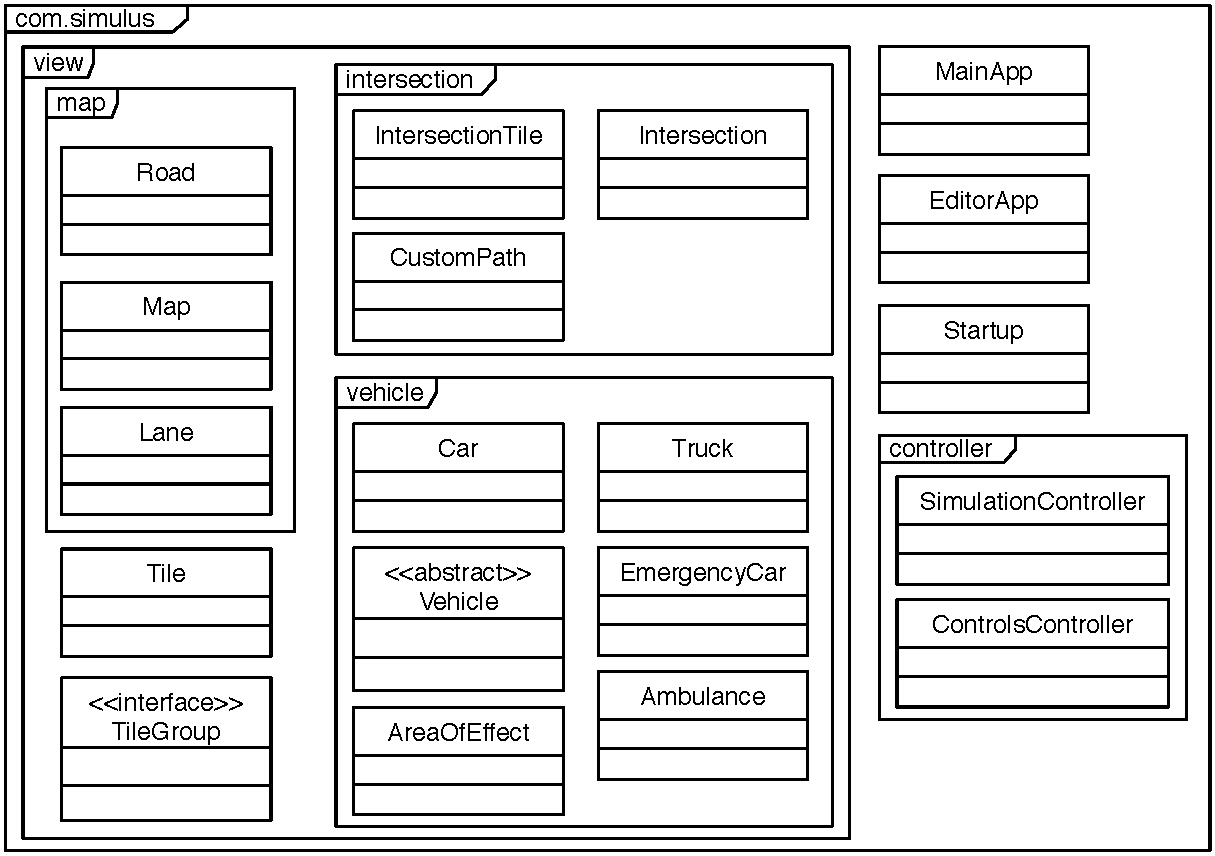
\includegraphics[width=\textwidth]{img/package_diagram.pdf}
		\caption[Snippet of the Package Diagram]{Snippet of the Package Diagram}
		\label{fig:packages}
	\end{center}
\end{figure}

Figure~\ref{fig:packages} shows an excerpt of the overall structure of the codebase. The package on the highest level of the hierarchy, \textit{com.simulus}, contains two subordinate packages besides three classes of itself. These three classes form the JavaFX application (and they all extend the JavaFX base class \textit{Application}). When the software suite is started, the \textit{Startup} class will present a splash screen that allows to choose between the simulator (\textit{MainApp}) and the map editor application (\textit{EditorApp}).
The \textit{controller} package then contains classes that do what its name in insinuates. The \textit{SimulationController} is responsible for the supervision of the running simulation and the modification of the simulation's parameters.  It also contains the definition of the \textit{AnimationThread} (Fig.~\ref{fig:animthread}) and manages said thread's lifecycle. The \textit{ControlsController} is the JavaFX controller class associated with the simulation parameter controls and the statistics on the right panel in the simulator application. 
The \textit{view} package contains three more subpackages and two classes on its own. The \textit{Tile} class forms the base for all the different types of tiles in the simulator, that includes land tiles, which are simply used to pretty up all tiles that are not part of the road network. A \textit{TileGroup} represents a collection of tiles, and is implemented by both \textit{Road} and \textit{Intersection}.  The three shown classes in the \textit{map} package are used to depict the map itself and the road network on it. \textit{Lane} objects are extensions of tiles. Each lane has a direction (north, south, east or west) and can be occupied by a vehicle. A \textit{Road} contains four lanes, either two north- and two southbound or two east- and two westbound lanes. The third class in the package, the \textit{Map}, is the actual representation of the road network. It contains the tile grid and exposes functionality to operate on this grid, e.g. calculating the average congestion of the network. Furthermore the map holds lists of all vehicles and traffic lights. \textit{Intersection}s are tilegroups as well, composed of \textit{IntersectionTiles}. These special tiles for intersections contain \textit{CustomPath}s, which allow for the above mentioned turning on intersections and are an extension to the JavaFX \textit{Path} class. They provide methods to check whether the path is free and whether the path should be available at all. A path can be unavailable if the intersection is not a four-way junction but for example a T-junction.  
In the \textit{vehicle} package we encapsulate all the different kinds of vehicles the simulator supports. The abstract class \textit{Vehicle} provides the basic functionality, i.e. accelerating, moving, avoiding obstacles and alike. \textit{Truck}s, \textit{Car}s and \textit{EmergencyCar}s then extend this class with their special behaviours and attributes. In order to produce the advanced functionality of an \textit{Ambulance}, this class is composed of an EmergencyCar and an \textit{AreaOfEffect}. This area of effect is a circle, surrounding the emergency car and depicts the range of an emerging ambulance's influence on other nearby traffic participants.

\subsubsection{Requirements}
Requirement 1a, the simulation of individual vehicles, means that the simulation has to evaluate the behaviour of each car individually and draw conclusions for the traffic systems based on these observations. In simulation terms, we derive macroscopic statistics of a traffic network based on the aggregation of microscopic data.

\begin{wrapfigure}{t}{0.3\textwidth}
	\begin{center}
		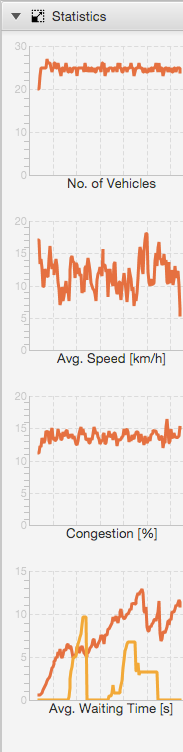
\includegraphics[scale=0.5]{img/graphs.png}
		\caption[Simulation Statistics at Runtime]{Simulation Statistics at Runtime}
		\label{fig:graphs}
	\end{center}
\end{wrapfigure}

During the simulation, vehicles enter the traffic network at one point, make their way through it, and exit it at an arbitrary touching-point of a road and the border of the map. (1b) On their way through the network, they exhibit different driving behaviours (1c), that is cautious drivers do not overtake and adjust their speed to surrounding cars while reckless drivers want to maximise their speed and overtake whenever possible. The third possible behaviour is called "semi". A car with this behavioural setting will change from cautious to reckless driving from time to time.

The observations of the traffic network mentioned above are captured in live statistics at runtime of the simulation (1d).  We provide four charts measuring different network statistics (Fig.~\ref{fig:graphs}). The first metric is the number of cars currently in the system, which gives a good reference point when analysing the trend of the other metrics. Secondly, we show the average speed of all present vehicles. The speed is given in km/h (cf. formula~\ref{for:speed} for the unit conversion) and presented as arithmetic mean. That is, $ n^{-1}\sum\limits_{i=1}^n v_i$ for $n$ vehicles on the map and vehicle $i$ moving with velocity $v_i$. The third chart displayed shows the current congestion in the traffic network. Congestion is defined as the fraction of currently occupied tiles and the total number of tiles: $\frac{|\:\lbrace \:t\:|\:t\:\epsilon\:T\:\wedge\:t\:is\:occupied\rbrace\:|}{|\:T\:|}$, $T$ being the set of tiles. The last chart depicts two data series. First, the average time a normal vehicle had to wait on its way through the map (red) and as a second line the average waiting time of an emergency vehicle (orange). This chart nicely illustrates how the the fact that surrounding vehicles give way for emergency vehicles reduces their idle time in the traffic network. The displayed time is translated from simulation time into real time (i.e. multiplied by factor 10). The average is again shown as the arithmetic mean as follows: $10*n^{-1}\sum\limits_{i=1}^n w_i$, $w_i$ being the amount of simulation ticks vehicle $i$ has been idle. For improved readability, the statistics can be popped out of the user interface into a separate, resizable window (see button in top bar in Fig.~\ref{fig:graphs}). Additionally, the suite allows the export of the current simulation session's statistics into the comma-separated-value format for further analysis.

When simulating the flow of cars in a traffic network it is of utmost importance to be able to alter the traffic management policies that are brought into effect (requirement 1e). Traffic management policies that are tangible in real-life situations include speed limits and the duration of red-light-phases of traffic lights. Besides these two, the Simulus simulation suite allows adjustment of the following simulation-specific policies: the maximum number of cars in the network, the tickrate of the simulation in milliseconds, the spawn delay, i.e. after how many ticks a new vehicle appears on the map, the ratio of cars to trucks (a value of 1 restricts trucks from spawning, 0 analogous stops cars from spawning), and lastly the ratio of reckless drivers to cautious drivers. All of the aforementioned but the traffic light duration are adjustable via sliders on the right side of the interface. The traffic light duration can be randomised for all traffic lights at once via a button, assigning a phase duration between 2000 and 5000 milliseconds.

The requirements discussed above comprised the \textit{Must have} category of our goals. The next requirement to mention is the implementation of emergency services (2a). Just like in real-life traffic emergency vehicles enjoy privileges in our simulation. In order to simulate the special attention that other drivers pay to approaching emergency vehicles, we introduce an "Area of Effect". This area, implemented as a circle, surrounds the moving ambulance. Any normal vehicle that intersects said circle will slow down to 10km/h and merge to an adjacent lane if it is in the same lane with the ambulance. If the vehicle intersects the area of effect but is currently in a lane adjacent to the ambulance it will slow down and keep a 3 tile (i.e. 15m) distance to cars in the front in order to allow other cars to merge into its lane. Emergency vehicles ignore red lights whenever the intersection is clear.

Why and how we accommodate user-defined maps (2b) will be discussed in length in section ~\ref{ss:req-editor}. The import and export of maps and settings (3a) is an optional requirement. We envisioned allowing users to define maps and store them in XML files to reuse or share them. Similarly, exporting and importing the simulation settings and policies used in a simulation session would allow recreating the exact session at a later point in time. Using external map sources to create maps, e.g. base a map on the the Google Maps representation online, enables users to simulate real-life traffic networks without the necessity of recreating them.

The last mentioned requirement, is stating what the software will not have: reused code or third-party libraries. We want to design and implement car's behaviours and the logic of the simulation on our own and not rely on external libraries.

\subsection{Editor}\label{ss:req-editor}

\begin{figure}[h]
	\begin{center}
		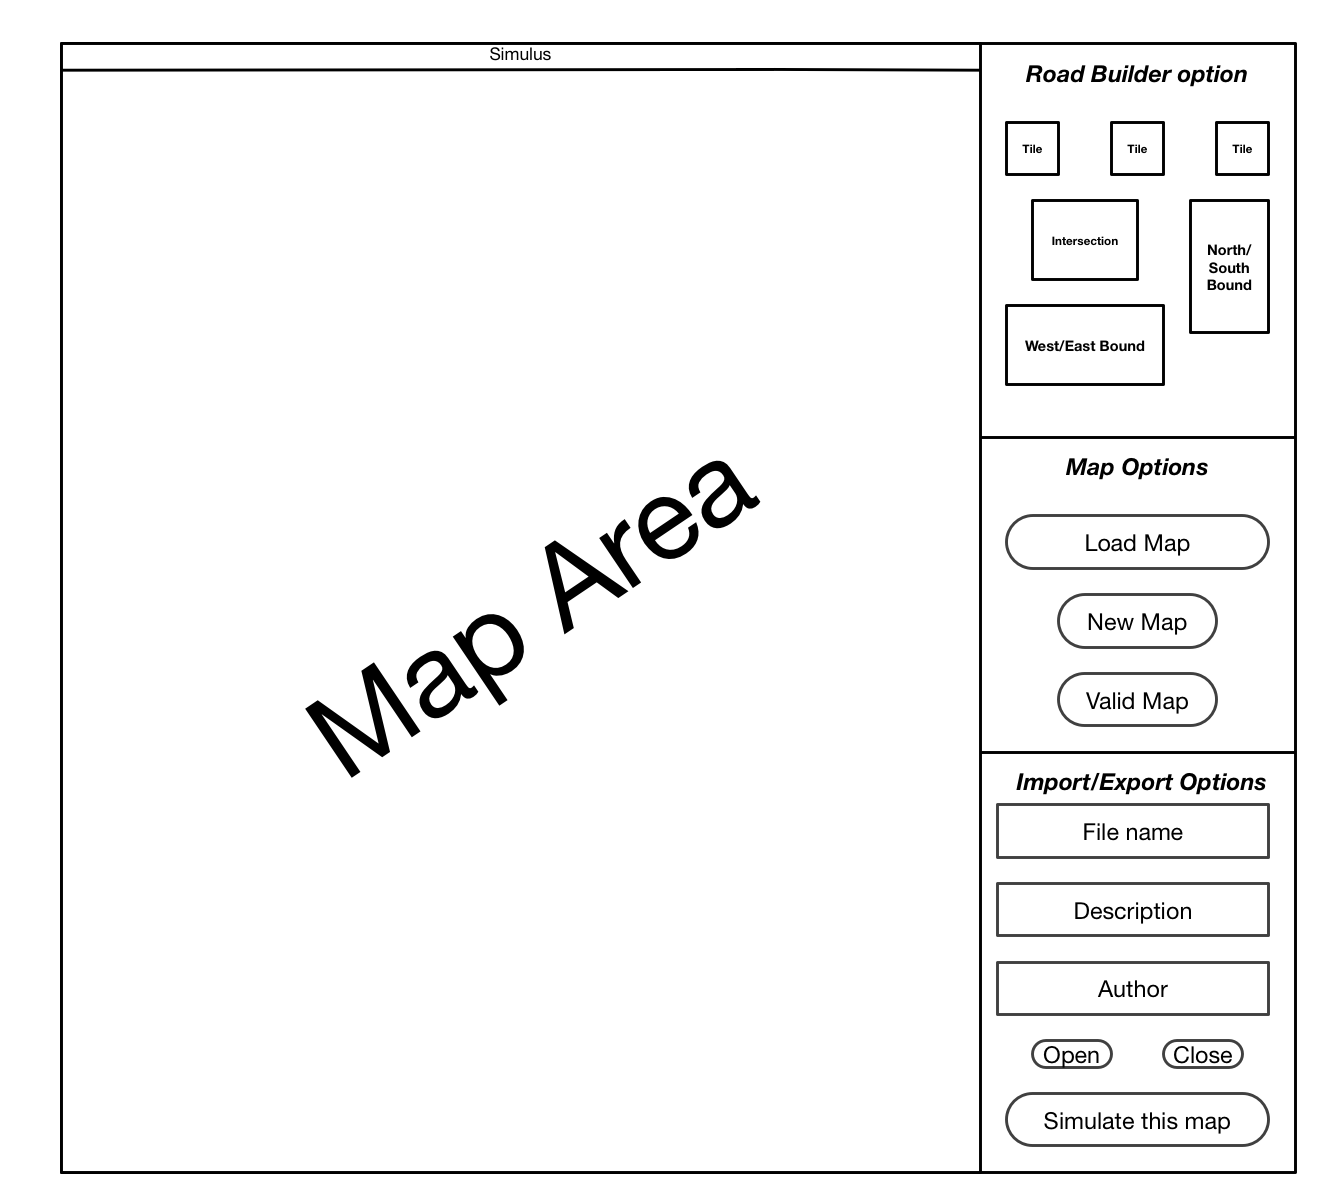
\includegraphics[width=\textwidth]{img/Map_Editor_Wireframe.png}
		\caption{Map Editor Wireframe}
		\label{fig:editorwireframe}
	\end{center}
\end{figure}


